\section{Design} \label{sec:design}

Analysis of the requirements described in section~\ref{sec:requirements} as well as those in \href{https://moodle.insttech.washington.edu/mod/resource/view.php?id=32929}{Lecture 16b} yielded the hierarchy shown in Figure~\ref{fig:hierarchy}.

\begin{figure}
    \centering
    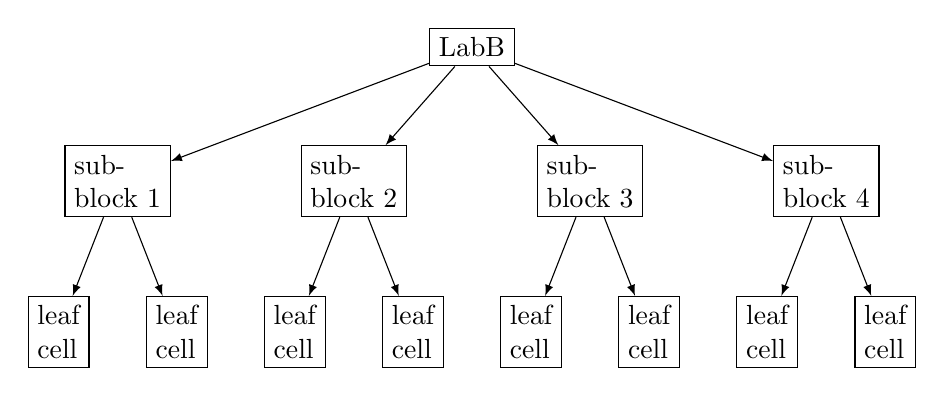
\begin{tikzpicture}[
            every node/.style={rectangle, align=left},
            level/.style={growth parent anchor=south, level distance=1cm},
            level 1/.style={sibling distance=3cm},
            level 2/.style={sibling distance=1.5cm},
            edge from parent/.style={draw,-latex},
            every child node/.style={anchor=north}]
        \node [draw] (top) {LabB}
            child {node [draw] (sub1) {sub-\\block 1}
                child {node [draw] (leaf1) {leaf\\cell}}
                child {node [draw] (leaf2) {leaf\\cell}}
            }
            child {node [draw] (sub2) {sub-\\block 2}
                child {node [draw] (leaf3) {leaf\\cell}}
                child {node [draw] (leaf4) {leaf\\cell}}
                        }
            child {node [draw] (sub3) {sub-\\block 3}
                child {node [draw] (leaf5) {leaf\\cell}}
                child {node [draw] (leaf6) {leaf\\cell}}
                        }
            child {node [draw] (sub4) {sub-\\block 4}
                child {node [draw] (leaf7) {leaf\\cell}}
                child {node [draw] (leaf8) {leaf\\cell}}
                        };
    \end{tikzpicture}
    \label{fig:topdown}
    \caption{Top-down Design Methodology}
\end{figure}